\begin{pastexam}[label={px:ntust-111-ice-08}]{臺科大資工所 111 學年度 第 8 題}
（問答）

About the graph: (10\%)
\begin{enumerate}[label=(\arabic*)]
\item Given an unweighted digraph, how many paths of length 4 are there from node $C$ to node $E$?
(5\%)

\begin{center}
\begin{tikzpicture}[font=\sffamily,n/.style={circle,draw,inner sep=0pt,minimum size=8mm},
  >={Stealth[length=2mm]}]
\node[n] (A) at (0.00,0.00) {A};
\node[n] (B) at (-1.65,-1.40) {B};
\node[n] (E) at (1.59,-1.50) {E};
\node[n] (C) at (-1.14,-3.13) {C};
\node[n] (D) at (1.05,-3.19) {D};
\draw[->] (B)--(A);
\draw[->] (A)--(E);
\draw[->] (B.20)--(E.165);
\draw[->] (A.250)--(C.60);
\draw[->] (D.115)--(A.295);
\draw[->] (C.120)--(B.268);
\draw[->] (B.305)--(C.88);
\draw[->] (D.150)--(B.355);
\draw[->] (C.15)--(E.200);
\draw[->] (C.310)--(D.218);
\draw[->] (D.88)--(E.235);
\draw[->] (E.268)--(D.50);
\end{tikzpicture}
\end{center}

\item Given an undirected connected graph, which nodes are the articulation points? (5\%)

\begin{center}
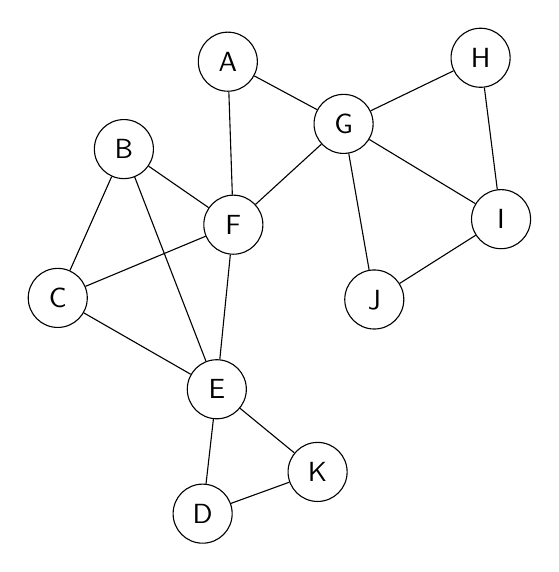
\begin{tikzpicture}[font=\sffamily,n/.style={circle,draw,inner sep=0pt,minimum size=7.5mm}]
\node[n] (A) at (0.00,0.00) {A};
\node[n] (H) at (3.21,0.05) {H};
\node[n] (G) at (1.47,-0.79) {G};
\node[n] (B) at (-1.32,-1.11) {B};
\node[n] (F) at (0.07,-2.07) {F};
\node[n] (I) at (3.47,-2.00) {I};
\node[n] (C) at (-2.16,-3.00) {C};
\node[n] (J) at (1.86,-3.02) {J};
\node[n] (E) at (-0.14,-4.16) {E};
\node[n] (K) at (1.14,-5.21) {K};
\node[n] (D) at (-0.32,-5.74) {D};
\draw (A)--(G) (A)--(F) (B)--(F) (B)--(C) (B)--(E) (C)--(F) (C)--(E) (F)--(G) (F)--(E) (G)--(H)
      (G)--(I) (G)--(J) (H)--(I) (I)--(J) (E)--(D) (E)--(K) (D)--(K);
\end{tikzpicture}
\end{center}
\end{enumerate}
\end{pastexam}

\begin{pastsoln}
答案：(1) $10$ 條；(2) $E$、$F$、$G$。

(1) 屬於資結書第~21~章（圖的表示），(2) 屬於第~23~章（割點）。

\textbf{(1)} 照資結書定義~21.1，路徑可以重複經過頂點，長度是邊數；要數的是 $C$ 出發、走 $4$ 條邊到 $E$ 的走法。
圖上的邊（$u \to v$）：
\[
A \to C, E;\quad B \to A, C, E;\quad C \to B, D, E;\quad D \to A, B, E;\quad E \to D.
\]
\textbf{方法一：鄰接矩陣的次方。} 設 $M$ 是鄰接矩陣（列、行依 $A, B, C, D, E$ 排），$(M^k)_{uv}$ 就是 $u$ 到 $v$
長度 $k$ 的路徑數：$(M^{k})_{uv} = \sum_w (M^{k-1})_{uw} M_{wv}$，最後一步從 $w$ 走到 $v$。 只要 $C$ 那一列：
\begin{center}
\begin{tabular}{ccccccl}
\toprule
$k$ & 到 $A$ & 到 $B$ & 到 $C$ & 到 $D$ & 到 $E$ & 怎麼算 \\
\midrule
$1$ & $0$ & $1$ & $0$ & $1$ & $1$ & $C$ 的出邊 \\
$2$ & $2$ & $1$ & $1$ & $1$ & $2$ & 例：到 $A$ 由 $B$、$D$ 各 $1$ \\
$3$ & $2$ & $2$ & $3$ & $3$ & $5$ & 例：到 $C$ 由 $A$ 的 $2$ 加 $B$ 的 $1$ \\
$4$ & $5$ & $6$ & $4$ & $8$ & $10$ & 到 $E$：$A, B, C, D$ 的 $2 + 2 + 3 + 3$ \\
\bottomrule
\end{tabular}
\end{center}
每一列由上一列算：到 $v$ 的數目是「上一列每個能走到 $v$ 的 $w$ 的數目」的和。 走得到 $E$ 的是 $A, B, C, D$，所以
第 $4$ 列到 $E$ 是 $2 + 2 + 3 + 3 = 10$。

\textbf{方法二：直接列出來}（用來核對）：
\[
\begin{gathered}
CBACE,\ CBCBE,\ CBCDE,\ CBEDE,\ CDACE,\\
CDBAE,\ CDBCE,\ CDEDE,\ CEDAE,\ CEDBE,
\end{gathered}
\]
共 $10$ 條。 如果題目的 path 指不重複頂點的簡單路徑，只有 $CDBAE$ 一條；照資結書的定義和「長度 $k$ 的路徑數用鄰接
矩陣 $k$ 次方」這個常考的算法，答案是 $10$。

\textbf{(2)} 割點是拿掉它（和它的邊）之後圖會不連通的頂點（資結書第~23.5~節）。 把圖拆成雙連通元件（資結書
第~23.6~節）比較好看：
\begin{itemize}
\item $\{B, C, E, F\}$：邊 $BC, BE, BF, CE, CF, EF$，四個點兩兩相連。
\item $\{D, E, K\}$：三角形。
\item $\{A, F, G\}$：三角形 $AF, AG, FG$。
\item $\{G, H, I, J\}$：環 $G, H, I, J$ 加上 $GI$。
\end{itemize}
每一塊裡拿掉任何一個點，剩下的仍然連通；同時屬於兩塊的點就是割點：$E$（$\{B,C,E,F\}$ 和 $\{D,E,K\}$）、
$F$（$\{B,C,E,F\}$ 和 $\{A,F,G\}$）、$G$（$\{A,F,G\}$ 和 $\{G,H,I,J\}$）。 直接驗證：拿掉 $E$，$\{D, K\}$ 和其他點分開；
拿掉 $F$，$\{B, C, E, D, K\}$ 和 $\{A, G, H, I, J\}$ 分開；拿掉 $G$，$\{H, I, J\}$ 和其他點分開。 其餘的點都只在一塊
裡，例如拿掉 $A$，$F$、$G$ 仍有邊 $FG$ 相連。
\end{pastsoln}
